\documentclass[
    12pt,
    a4paper,
    addpoints,
    answers,
    convocatoria=ext,
    titulacion=NoCD,
    curso=2024/2025,
]{db-exam}

\begin{document}

\begin{questions}

\question[2\half] Modelado entidad relación

Realizar un modelo conceptual de datos mediante la técnica del modelo \textbf{Entidad Relación de Chen} teniendo en cuenta la siguiente descripción:

\begin{quotation}
La organización EURO-NCAP es la entidad Europea de referencia encargada de evaluar y certificar la seguridad de vehículos a motor de distintas marcas y modelos mediante la realización de pruebas especializadas. Se fundó con el objetivo de mejorar los estándares de seguridad vial en Europa, de forma que se pudiera garantizar que los vehículos comercializados cumplieran con los requisitos más exigentes en materia de protección de los ocupantes y peatones. Para ello, EURO-NCAP, en colaboración con fabricantes, organismos reguladores y laboratorios independientes, diseña y ejecuta un conjunto de pruebas especializadas que abarcan distintos aspectos de la seguridad del vehículo, como, por ejemplo, la resistencia estructural, la eficacia de los sistemas de retención o el comportamiento ante colisiones.

Cada vez que un vehículo, identificado por su marca y modelo, es sometido a una de estas pruebas, se registra la calificación obtenida y la fecha en la que se realizó. Las pruebas se identifican por un nombre y tienen una duración determinada y un protocolo específico por el cual se rigen. Es importante destacar que un mismo vehículo puede participar en varias pruebas a lo largo de su vida, ya sea para evaluar diferentes aspectos de su seguridad o para comprobar mejoras introducidas por el fabricante. Asimismo, una misma prueba puede ser aplicada a diferentes vehículos, lo que permite comparar resultados y establecer clasificaciones entre modelos.

Cada vehículo está compuesto por diversos componentes, como el \textit{air-bag}, los frenos o el chasis, de los que se desea almacenar su nombre, que será único, y su descripción. Cada componente puede encontrarse en uno o más vehículos. Además, algunos componentes pueden estar formados a su vez por otros componentes del mismo vehículo.

En la realización de las pruebas participan ingenieros e ingenieras que pueden intervenir en varias pruebas y desempeñar diferentes roles en cada una de ellas (supervisor/a, técnico/a u observador/a). De cada ingeniero/a se conoce un identificador único, su nombre y su especialidad profesional. Es fundamental poder registrar no solo quien han participado en cada prueba, sino también el rol concreto que han desempeñado en cada una de ellas.

Por otro lado, cada componente puede estar asociado a uno o varios certificados de calidad. Un certificado de calidad tiene un número identificador (que puede repetirse) y una fecha de emisión, pero depende del componente al que está asociado, ya que un mismo número de certificado puede repetirse en componentes de distintos vehículos. Es necesario poder registrar los certificados de calidad de cada componente, así como la fecha en la que fueron emitidos.

Ante la complejidad y el volumen de información que maneja, la organización EURO-NCAP desea disponer de un sistema de información robusto y flexible que permita gestionar todos estos datos de manera estructurada. Este sistema debe facilitar la consulta y el análisis de las pruebas realizadas, las calificaciones obtenidas por los vehículos, la composición detallada de los vehículos y sus componentes, los certificados de calidad asociados a cada componente, así como la participación de los ingenieros en las distintas pruebas y los roles que han desempeñado. De este modo, EURO-NCAP podrá optimizar sus procesos de evaluación, mejorar la transparencia de sus resultados y contribuir de manera más eficaz a la seguridad vial en Europa.
\end{quotation}

Se pide realizar un \textbf{modelo entidad-relación de Chen} justificando las  \textbf{cardinalidades mínimas} de al menos dos relaciones (\textbf{ambos lados de la relación}).

\begin{solution}[50em]
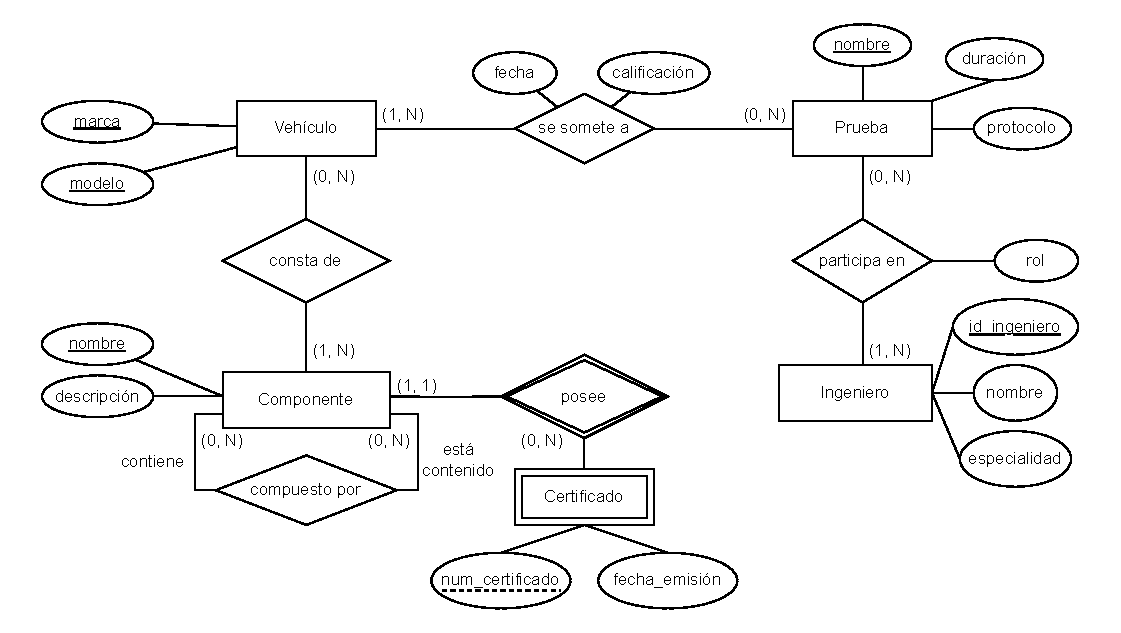
\includegraphics[width=\textwidth]{figs/bbdd-2024-2025-extraordinaria/mer25ex.pdf}

Cardinalidades mínimas:
\begin{itemize}
    \item La cardinalidad mínima de vehículo con respecto a prueba es 1, ya que un vehículo no se registra en el sistema hasta ser sometido a alguna prueba. Por otra parte, la cardinalidad mínima de prueba con respecto a vehículo es 0, pues es posible definir una prueba y almacenarla en el sistema antes de haber sometido ningún vehículo a la misma.
    \item La cardinalidad mínima de componente con respecto a certificado es 0, pues puede haber componentes que no dispongan de ningún certificado. Por otra parte, la cardinalidad mínima de certificado con respecto a componente es 1, pues no puede existir un certificado sin estar asociado a un componente.
\end{itemize}
\end{solution}

\newpage
\question[1\half] Dado el siguiente modelo relacional\footnote{Tenga en cuenta que las claves primarias aparecen \underline{subrayadas} mientras que las claves foráneas aparece en \textit{cursiva} junto con el superíndice \textsuperscript{FK} y comparten nombre con la clave primaria a la que referencian.} que representa la base de datos de las pruebas Euro-NCAP de seguridad de los vehículos ante colisiones:

\texttt{VEHICULO (\underline{idV}, marca, modelo)}

\texttt{PRUEBA (\underline{idP}, tipo, duracion)}

\texttt{PUNTUACION (\underline{\textit{idV}}\textsuperscript{FK}, \underline{\textit{idP}}\textsuperscript{FK}, \underline{fecha}, calificacion)} 

Donde \texttt{calificación} tendrá un valor entre 1 y 5 y se refiere a las estrellas obtenidas en la prueba correspondiente.

Se pide dar respuesta con álgebra relacional a las siguientes cuestiones:
\begin{parts}
\part[\half] ``\textit{Obtener el identificador de aquellos vehículos que hayan pasado con al menos 3 estrellas todas las pruebas que existen}''.
\begin{solution}[12em]

$\Pi_{idV, idP}(\sigma_{\text{calificación>=3}} (PUNTUACION) ) \div  \Pi_{idP} (PRUEBA) $

\end{solution}
\part[\half] ``\textit{Obtener el identificador de aquellos vehículos que hayan pasado con al menos 3 estrellas todas las pruebas a las que han sido sometidos}''.
\begin{solution}[12em]

$\Pi_{idV}(PUNTUACION)  - \Pi_{idV} [\sigma_{\text{calificación<3}}(PUNTUACION)] $

\end{solution}

\part[\half] ``\textit{Obtener las marcas que tengan algún vehículo que haya sido sometido tanto a la prueba de tipo 'choque frontal' como a la de tipo 'choque lateral'}''.
\begin{solution}[12em]

$\Pi_{marca} [ VEHICULO \bowtie ( $

$\Pi_{idV} [\sigma_{\text{tipo='choque frontal'}}(PRUEBA \bowtie PUNTUACION)] $

$\cap$

$\Pi_{idV} [\sigma_{\text{tipo='choque lateral'}}(PRUEBA \bowtie PUNTUACION)] $

$)]$

\end{solution}


\end{parts}



\newpage
\question[4] Dado el siguiente modelo relacional\footnote{Tenga en cuenta que las claves primarias aparecen \underline{subrayadas} mientras que las claves foráneas aparece en \textit{cursiva} junto con el superíndice \textsuperscript{FK} y comparten nombre con la clave primaria a la que referencian.} ampliado y modificado de la base de datos Euro-NCAP del Ejercicio 2:

\texttt{FABRICANTE (\underline{idF}, marca, pais)}

\texttt{PLANTA\_PRODUCCION (\underline{\textit{idF}}\textsuperscript{FK}, \underline{numero}, capacidad, localizacion)}

\texttt{VEHICULO (\underline{idV}, modelo, año, \textit{idF}\textsuperscript{FK}, \textit{numero}\textsuperscript{FK})}

\texttt{PRUEBA (\underline{idP}, tipo, duracion)}

\texttt{PUNTUACION (\underline{\textit{idV}}\textsuperscript{FK}, \underline{\textit{idP}}\textsuperscript{FK}, \underline{fecha}, calificacion)} 

Se pide dar respuesta a las siguientes cuestiones:

\begin{parts}

\part[\half] Resuelva mediante SQL la siguiente consulta: ``\textit{obtener todos los datos de los fabricantes que no han fabricado ningún vehículo en plantas de producción ubicadas en Madrid}''.
\begin{solution}[20em]
\begin{lstlisting}[language=SQL]
SELECT *
FROM FABRICANTE f
WHERE f.idF NOT IN 
  (SELECT DISTINCT v.idF
   FROM VEHICULO v
   INNER JOIN PLANTA_PRODUCCION pp 
        ON v.idF = pp.idF AND v.numero = pp.numero
   WHERE pp.localizacion = 'Madrid');
\end{lstlisting}
\end{solution}

\part[\half] Resuelva mediante SQL la siguiente consulta: ``\textit{obtener los vehículos (identificador) del año 2023, junto con la marca de su fabricante, y su calificación promedio en pruebas de calidad, de aquellos vehículos con una calificación promedio igual o superior a 4, mostrando los resultados ordenados según la calificación promedio de forma descendente}''.
\begin{solution}[20em]
\begin{lstlisting}[language=SQL]
SELECT v.idV, f.marca, AVG(p.calificacion) AS puntuacion_media
FROM FABRICANTE f
  INNER JOIN VEHICULO v 
    ON v.idF = f.idF
  INNER JOIN PUNTUACION p 
    ON v.idV = p.idV 
WHERE v.año = 2023
GROUP BY v.idV, f.marca
HAVING puntuacion_media >= 4 
ORDER BY puntuacion_media DESC;
\end{lstlisting}
\end{solution}

\newpage

\part[\half] Resuelva mediante SQL la siguiente consulta: ``\textit{obtener el identificador de la fábrica, su número, y localización de aquellas plantas de producción en las que se ha fabricado algún vehículo al que se le ha realizado todas las pruebas de tipo `choque lateral' }''.
\begin{solution}[30em]
\begin{lstlisting}[language=SQL]
SELECT pp.idF, pp.numero, pp.localizacion
FROM PLANTA_PRODUCCION pp 
  INNER JOIN VEHICULO v 
    ON v.idF = pp.idF AND v.numero = pp.numero
WHERE v.idV IN (SELECT v.idV
                FROM VEHICULO v  
                   INNER JOIN PUNTUACION P 
                        ON p.idV = v.idV
                   INNER JOIN PRUEBA pru 
                        ON pru.idP = p.idP 
                WHERE pru.tipo = 'choque lateral'
                GROUP BY v.idV 
                HAVING COUNT(DISTINCT p.idP) = (SELECT COUNT(*)
                                                FROM PRUEBA
                                                WHERE tipo = 'choque lateral'
                                                )
                );
\end{lstlisting}
\end{solution}

\part[\half] Escriba una sentencia en SQL que cree la tabla VEHICULO tal y como está definida en el enunciado.
\begin{solution}[35em]
\begin{lstlisting}[language=SQL]
CREATE TABLE VEHICULO (
    idV INTEGER NOT NULL,
    modelo VARCHAR(128) NOT NULL,
    año INTEGER NOT NULL,
    idF INTEGER NOT NULL,
    numero INTEGER NOT NULL,
    PRIMARY KEY(idV),
    FOREIGN KEY(idF, numero) REFERENCES PLANTA_PRODUCCION(idF, numero)
)
\end{lstlisting}\end{solution}

\newpage 

\part[\half] Escribir una \textbf{FUNCIÓN} denominada \texttt{contar\_vehiculos} que dados como parámetros el identificador de un fabricante (\texttt{idFabricante}) de tipo \texttt{VARCHAR(3)} y el año de fabricación, devuelva en un \texttt{INTEGER} el número de coches fabricados por el fabricante en el año indicado.

\begin{solution}[67em]
\begin{lstlisting}[language=SQL]
DELIMITER $$
CREATE FUNCTION contar_vehiculos (idFabricante VARCHAR(3), añoFabricacion INTEGER)
RETURNS INTEGER
DETERMINISTIC
BEGIN
    DECLARE conteo INTEGER;
    
    SELECT COUNT(*) INTO conteo
    FROM vehiculo
    WHERE idF = idFabricante AND año = añoFabricacion;
    
    RETURN conteo;
END$$
DELIMITER ;
\end{lstlisting}
\end{solution}

\newpage 

\part[1] Escribe un \textbf{PROCEDIMIENTO} denominado \texttt{listar\_ventas} que liste el desglose anual de vehículos fabricados por los fabricantes de un país específico durante un año determinado. Tanto el país como el año deben proporcionarse como parámetros de entrada de tipos \texttt{VARCHAR(50)} e \texttt{INTEGER} respectivamente. El listado debe devolverse mediante un parámetro de salida de tipo \texttt{VARCHAR(1000)} en el que se indicará, para cada fabricante del país, el nombre del fabricante (\texttt{marca}) y el número total de vehículos producidos en ese año. El formato del listado debe ser el siguiente: \texttt{MarcaA:23|MarcaB:8|...|MarcaZ:42}. Los fabricantes de este listado deben aparecer ordenados alfabéticamente. Será obligatorio emplear la función \texttt{contar\_vehiculos} del ejercicio anterior así como el uso de un \texttt{CURSOR} para implementar este procedimiento. Adicionalmente, se puede utilizar la función \texttt{CONCAT}\footnote{La función \texttt{CONCAT} permite concatenar varias cadenas de texto. Por ejemplo, \texttt{CONCAT(`a',`b',`c')} devuelve la cadena \texttt{`abc'}.} para concatenar las cadenas que formen el listado de salida.

\begin{solution}[56em]
\begin{lstlisting}[language=SQL]
DELIMITER $$
CREATE PROCEDURE listar_ventas (IN pais_fabricacion VARCHAR(50), IN año INTEGER, OUT cadena VARCHAR(1000))
BEGIN
    DECLARE marcaFabricante VARCHAR(50);
    DECLARE cantidad INTEGER;
    DECLARE primero INT DEFAULT TRUE;
    DECLARE hecho INT DEFAULT FALSE;
    DECLARE cur CURSOR FOR SELECT marca, contar_vehiculos(idF, año)
                           FROM vehiculo
                               NATURAL JOIN fabricante
                           WHERE pais = pais_fabricacion
                           ORDER BY marca ASC;
    DECLARE CONTINUE HANDLER FOR NOT FOUND SET hecho = TRUE;
    
    OPEN cur;
    read_loop: LOOP
        FETCH cur INTO marcaFabricante, cantidad;
        IF hecho THEN
            LEAVE read_loop;
        END IF;

        IF primero THEN
            SET cadena = CONCAT(marcaFabricante,':',cantidad); 
            primero = FALSE;
        ELSE
            SET cadena = CONCAT(cadena, '|', marcaFabricante,':',cantidad);
        END IF;
    END LOOP;
    CLOSE cur;
END$$
DELIMITER ;

\end{lstlisting}        
\end{solution}

\newpage

\part[\half] Se quiere evitar, mediante un \textbf{TRIGGER}, la fabricación de nuevos vehículos del fabricante con identificador \texttt{F16} en las plantas ubicadas en en Estados Unidos (\texttt{localizacion = `Estados Unidos'}). Codifica dicho TRIGGER.
\begin{solution}
\begin{lstlisting}[language=SQL]

DELIMITER $$
CREATE TRIGGER evitarFabricacionEstadosUnidos BEFORE INSERT ON vehiculo
FOR EACH ROW
BEGIN
    DECLARE localizacion_planta VARCHAR(50);

    SELECT localizacion INTO localizacion_planta
    FROM planta_produccion
    WHERE idF = NEW.idF AND numero = NEW.numero;

    IF NEW.idF = 'F16' AND localizacion_planta = 'Estados Unidos' THEN
            SIGNAL SQLSTATE '04000'
            SET MESSAGE_TEXT = 'No se permite la fabricacion de nuevos vehiculos del fabricante F16 en Estados Unidos';
    END IF;
END$$
DELIMITER ;

\end{lstlisting}       
\end{solution}
\end{parts}

\newpage

\question[2] Una clínica veterinaria \textit{SOS Bigotes Urgentes}, con varios centros en España, necesita migrar su sistema de gestión de datos desde un modelo relacional (SQL) a una base de datos NoSQL de documentos (json). Su modelo de datos actual es el que muestra el siguiente modelo relacional\footnote{Tenga en cuenta que las claves primarias aparecen \underline{subrayadas} mientras que las claves foráneas aparece en \textit{cursiva} junto con el superíndice \textsuperscript{FK} y comparten nombre con la clave primaria a la que referencian.}:


\texttt{CLINICA (\underline{idClinica}, nombre, direccion, telefono)}

\texttt{VETERINARIO (\underline{idVeterinario}, nombre, especialidad, \textit{idClinica}\textsuperscript{FK})}

\texttt{MASCOTA (\underline{idMascota}, nombre, especie, edad, \textit{idCliente}\textsuperscript{FK})}

\texttt{CLIENTE (\underline{idCliente}, nombre, telefono, \textit{idClinica}\textsuperscript{FK})}

En una primera migración usa un \textbf{modelo embebido} con una única colección con esta estructura:

\begin{lstlisting}[basicstyle=\scriptsize\ttfamily]
 clinicas: [
    {
      "_id": "clin001",
      "nombre": "Clinica Patas Felices",
      "direccion": "Calle del Hueso 42",
      "telefono": "555-123456",
      "veterinarios": [
        {
          "idVeterinario": "vet001", "nombre": "Dr. Lamepatas", "especialidad": "Cardiologia"
        },
        {
          "idVeterinario": "vet002", "nombre": "Dra. Ronroneo", "especialidad": "Dermatologia Felina"
        }
      ],
      "clientes": [
        {
          "idCliente": "cli001",
          "nombre": "Angeles Mai",
          "telefono": "600-111222",
          "mascotas": [
            {
              "idMascota": "m001", "nombre": "Baghera", "especie": "Gato", "edad": 5
            },
            {
              "idMascota": "m002", "nombre": "PdCar", "especie": "Gato", "edad": 3
            }
          ]
        },
        {
          "idCliente": "cli002",
          "nombre": "Carlos Ruiz",
          "telefono": "600-333444",
          "mascotas": [
            {
              "idMascota": "m003", "nombre": "Blu", "especie": "Perro", "edad": 2
            },
            {
              "idMascota": "m004", "nombre": "Bay", "especie": "Perro", "edad": 4
            }
          ]
        }
      ]
    }
 ]
\end{lstlisting}

\newpage
\begin{parts}
\part[1] Se pide diseñar la base de datos utilizando un modelo referenciado.
\begin{solution}[70em]
\begin{lstlisting}
// Clinicas 
[
    {
      "idClinica": "clin001",
      "nombre": "Clinica Patas Felices",
      "direccion": "Calle del Hueso 42",
      "telefono": "555-123456"
    }
]

// Veterinarios
[
  {
    "idVeterinario": "vet001",
    "nombre": "Dr. Lamepatas",
    "especialidad": "Cardiologia",
    "idClinica": "clin001"
  },
  {
    "idVeterinario": "vet002",
    "nombre": "Dra. Ronroneo",
    "especialidad": "Dermatologia Felina",
    "idClinica": "clin001"
  }
]

// Clientes
[
    {
      "idCliente": "cli001",
      "nombre": "Angeles Mai",
      "telefono": "600-111222",
      "idClinica": "clin001"
    },
    {
      "idCliente": "cli002",
      "nombre": "Carlos Ruiz",
      "telefono": "600-333444",
      "idClinica": "clin001"
    }
]

// Mascostas
[
  {
    "idMascota": "m001",
    "nombre": "Baghera",
    "especie": "Gato",
    "edad": 5,
    "idCliente": "cli001"
  },
  {
    "idMascota": "m002",
    "nombre": "PdCar",
    "especie": "Gato",
    "edad": 3,
    "idCliente": "cli001"
  },
  {
    "idMascota": "m003",
    "nombre": "Blu",
    "especie": "Perro",
    "edad": 2,
    "idCliente": "cli002"
  },
  {
    "idMascota": "m004",
    "nombre": "Bay",
    "especie": "Perro",
    "edad": 4,
    "idCliente": "cli002"
  }
]

\end{lstlisting}       
\end{solution}

\part[1] Contestar a las siguientes preguntas, indicando embebido o referenciado, justificando la respuesta:

\begin{subparts}
\subpart Si la aplicación requiere consultas frecuentes que recuperan toda la información de una clínica (incluyendo veterinarios, clientes y mascotas) en una sola operación, ¿qué modelo es más eficiente?
\begin{solution}[10em]
Embebido. Consultas únicas sin joins.
\end{solution}

\subpart Si se espera que la clínica tenga miles de clientes y mascotas, ¿qué diseño evitaría problemas de tamaño de documento y permitiría un crecimiento sostenible?
\begin{solution}[10em]
Referenciado, escala mejor con datos masivos.
\end{solution}

\subpart Si la especialidad de un veterinario cambia frecuentemente y hay que actualizarla en todos los registros asociados, ¿qué modelo simplificaría este proceso?
\begin{solution}[10em]
Referenciado: Actualización en un solo lugar. 
\end{solution}

\subpart Si un cliente puede llevar sus mascotas a múltiples clínicas, ¿qué modelo manejaría mejor esta relación sin duplicar datos?
\begin{solution}[10em]
Referenciado: Usar referencias evita redundancia.  
\end{solution}

\end{subparts}

\end{parts}

\end{questions}
\end{document}
